\documentclass[12pt, letterpaper]{article}
\usepackage[titletoc,title]{appendix}
\usepackage{color}
\usepackage{booktabs}
\usepackage[usenames,dvipsnames,svgnames,table]{xcolor}
\definecolor{dark-red}{rgb}{0.75,0.10,0.10} 
\usepackage[margin=1in]{geometry}
\usepackage[linkcolor=dark-red,
			colorlinks=true,
			urlcolor=blue,
			pdfstartview={XYZ null null 1.00},
			pdfpagemode=UseNone,
			citecolor={dark-red},
			pdftitle={Downweighting}]{hyperref}

\usepackage[resetlabels,labeled]{multibib}
\newcites{SI}{SI References}
\usepackage{natbib}

\usepackage{float}

\usepackage{geometry} % see geometry.pdf on how to lay out the page. There's lots.
\geometry{letterpaper}               % This is 8.5x11 paper. Options are a4paper or a5paper or other... 
\usepackage{graphicx}                % Handles inclusion of major graphics formats and allows use of 
\usepackage{amsfonts,amssymb,amsbsy}
\usepackage{amsxtra}
\usepackage{verbatim}
\setcitestyle{round,semicolon,aysep={},yysep={;}}
\usepackage{setspace}		     % Permits line spacing control. Options are \doublespacing, \onehalfspace
\usepackage{sectsty}		     % Permits control of section header styles
\usepackage{lscape}
\usepackage{fancyhdr}		     % Permits header customization. See header section below.
\usepackage{url}                     % Correctly formats URLs with the \url{} tag
\usepackage{fullpage}		%1-inch margins
\usepackage{multirow}
\usepackage{rotating}
\setlength{\parindent}{3em}

\usepackage[T1]{fontenc}
\usepackage{bm}
\usepackage{palatino}

\usepackage{chngcntr}

\def\citeapos#1{\citeauthor{#1}'s (\citeyear{#1})}

\makeatother


% Caption
\usepackage[hang, font=small,skip=0pt, labelfont={bf}]{caption}
%\captionsetup[subtable]{font=small,skip=0pt}
\usepackage{subcaption}

% tt font issues
% \renewcommand*{\ttdefault}{qcr}
\renewcommand{\ttdefault}{pcr}

\setcounter{page}{0}

\usepackage{lscape}
\renewcommand{\textfraction}{0}
\renewcommand{\topfraction}{0.95}
\renewcommand{\bottomfraction}{0.95}
\renewcommand{\floatpagefraction}{0.40}
\setcounter{totalnumber}{5}
\makeatletter
\providecommand\phantomcaption{\caption@refstepcounter\@captype}
\makeatother

\title{Explaining Partisan Affect: Partisan Response to Partisan Response}

\author{Douglas J. Ahler\thanks{Assistant Professor of Political Science, Florida State University, \href{mailto:dahler@fsu.edu}{\texttt{dahler@fsu.edu}}} \and Carolyn E. Roush\thanks{Democracy Postdoctoral Fellow, the Ash Center for Democratic Governance and Innovation at the Harvard Kennedy School, \href{mailto:carolyn_roush@hks.harvard.edu}{\texttt{carolyn\_roush@hks.harvard.edu}}} \and Gaurav Sood\thanks{Independent researcher, \href{gsood07@gmail.com}{\texttt{gsood07@gmail.com}}}}

\begin{document}
\maketitle
\thispagestyle{empty}

\begin{abstract}

\noindent 

\end{abstract}

\newpage
\doublespacing

\section*{Pilot: Partisan Response to Partisan Response to Scandals}

Does observation of outparty bias exacerbate affective polarization? Answering this question using observational data is difficult. Because partisans themselves interpret facts and events in a biased manner, disentangling the effect of one's own biased reasoning from any effect of observing the \textit{other party's} biased reasoning is near impossible. To circumvent this problem, we rely upon a randomized, controlled experiment to determine if and how partisans' exposure to out-party bias exacerbates the negative feelings they hold toward their opponents. Specifically, we use a series of vignettes about real political scandals and manipulate whether or not co-partisans responded to the scandal in an unbiased manner. This design holds constant both the scandal and the elite embroiled in the scandal, which helps to rule out important confounding variables that could muddle inferences drawn from observational data.

We focus on scandals (and partisans' reaction to them) in this experiment for a few reasons. For one, scandals are an easy way for citizens to hold politicians accountable for their actions. Typically, political accountability is assessed one of two ways:  (1) whether elected officials espouse and pursue the policies favored by their constituents and/or (2) whether elected officials contribute positively to government performance (most commonly assessed by economic outcomes). Evaluating politicians on these bases requires a certain level of political sophistication and objectivity that most ordinary citizens lack. As a result, people quite frequently fail to hold elected officials accountable using these metrics \citep[e.g.,][]{achen2016democracy,Bartels2008,healylenz_2014,Lenz2012,snidermanstiglitz_2012,soodiyengar_2014}. The Evaluating a scandal, on the other hand, requires much less effort. For one, voters do not have to proactively search for information about scandals; they are covered extensively by the media, and in particular by outlets that are ideologically dissimilar from the embroiled politician \citep{budaketal_2016,puglisisnyder_2011}. Secondly, scandals tend to focus on norm violations that are considered controversial outside the realm of politics,\footnote{A content analysis of political scandals between 2005 and 2011 suggests that the vast majority of scandals involve sexual behavior, substance abuse, corruption or malfeasance, or racist speech or behavior \citep{ahlersood_2014}.} making them easier for people to evaluate than other complex policies or issues. Because scandals are salient and relatively easy to comprehend, a partisan-motivated reaction to a one is likely to strike out-partisans as particularly egregious. Accordingly, we might expect citizens who observe a biased out-party response to a scandal to feel more negatively toward the other side as a result. 

To test this theory, we recruited 930 people to participate in a survey administered through Amazon's Mechanical Turk in November 2013. To preclude suspicion, we told respondents they would be participating in a broad survey on political media consumption and political learning. Prior to our experiment, we posed a question to determine whether or not respondents were paying attention to the survey. In particular, the question asked respondents to mark two particular responses. Of the 930 respondents, 38 respondents failed to complete the task as requested. We removed these participants from our sample as we felt that they were merely adding noise to the data. Because we are interested in \textit{partisans'} reactions to an observed response (or lack thereof) to party scandals, we further limit our analysis to responses from self-identified and leaning partisans.\footnote{We group together ``leaning'' Independents with ``strong'' and ``weak'' partisans, based on previous research suggesting Independent leaners think and behave similarly to partisans \citep{keithetal_1992}.} Of the 726 self-identified and leaning partisans, 552 are Democrats, consistent with the general liberal bias in MTurk samples \citep{BerinskyHuberLenz2012}. 

Participants were randomly assigned to read a news story on one of three contemporary political scandals: (1) the troubled rollout of the U.S. health exchange website, Healthcare.gov (which we classify as a Democratic Party scandal), (2) Senator Ted Cruz's controversial decision to force a government shutdown (which we classify as a Republican Party scandal), and (3) Toronto mayor Rob Ford's drug scandal (our "control" condition). We selected these the Cruz and Healthcare.gov cases because they were timely examples of real-world, high-profile missteps that generated significant news coverage. Within these two experimental groups, we further manipulated whether Democratic (Republican) Party supporters' opinions of Obama (Cruz) changed in response to the blunder. This created five conditions based on vignette content:  (1) \textit{Democrats - Response}, in which Democrats show less support for Obama post-scandal, (2) \textit{Democrats - No Response}, in which Democrats maintain high support for Obama post-scandal, (3) \textit{Republicans - Response}, in which Republicans show less support for Cruz post-scandal, (4) \textit{Republicans - No Response}, in which Republicans maintain high support for Cruz post-scandal, and (5) \textit{Control.} (See Appendix A1 for vignettes.) After exposing respondents to these stories, we asked them to rate the Democratic and Republican parties using feeling thermometers. We use party feeling thermometer scores as our dependent variables in this study because they are the most common means by which to measure affective polarization \citep[e.g.,][]{haidthetherington_2012,hetheringtonrudolph_2015,IyengarSoodLelkes2012,iyengarwestwood_2014,mason_2015}. 

Though our sample is disproportionately Democratic, we analyze the results of our experiment separately among Democrats and Republicans to detect any partisan differences in response to the treatments. We also elect to analyze the feeling thermometers as separate dependent variables, as previous research demonstrates that the growing gulf in partisan affect has been caused primarily by increasing dislike of the out-party and not by a corresponding increase in warm in-party feelings \citep{haidthetherington_2012, IyengarSoodLelkes2012}. As out-party negativity is the prime mover over time, we might also expect our experiments to produce greater variation in the out-party feeling thermometers compared to the in-party feeling thermometers. Accordingly, our analysis produces four OLS regressions that analyze the impact of our experimental manipulation on out- and in-party affect among Democrats and Republicans. 

For each model, we include four dummy variables representing assignment to one of our experimental conditions - (1) \textit{Out-Party - Response} (\textit{Democrats - Response} for Republicans; \textit{Republicans - Response} for Democrats); (2) \textit{Out-Party - No Response} (\textit{Democrats - No Response} for Republicans; \textit{Republicans - No Response} for Democrats); (3) \textit{In-Party - Response} (\textit{Democrats - Response} for Democrats and \textit{Republicans - Response} for Republicans); and (4) \textit{In-Party - No Response} (\textit{Democrats - No Response} for Democrats and \textit{Republicans - No Response} for Republicans).\footnote{\textit{Control} is omitted as the reference category.} Respondents receive a value of 1 if they were assigned to that particular condition and a value of 0 if they were not. The dependent variables --- the in- and out-party feeling thermometers --- range from 0 to 100. Positive coefficients indicate an increase in warmth toward the party in question; negative coefficients indicate a decrease in warmth toward the party in question.

Given our theory that partisans respond disproportionately to out-party bias and that observation of out-party bias heightens negative feelings toward the other side, we expect the largest experimental effects to appear among those respondents assigned to the \textit{Out Party - Response} or \textit{Out-Party - No Response} conditions. It is our expectation that observing a lack of response to a scandal on the part of the other side (\textit{Out-Party - No Response}) increases negative affect toward the out party (meaning that coefficients in these conditions should be negative). Conversely, those partisans who observe the other side reacting in a ``nonbiased'' manner --- those assigned to the \textit{Out-Party - Response} --- should feel, on average, more warmly toward their opponents, since the vignette suggests that their political opponents are more rational than anticipated. We have fewer expectations about how our experiment might affect people's feelings toward their own side. Since we argue partisans' response to bias is asymmetric, we do not expect information about whether one's own side engaged or did not engage in motivated reasoning to meaningfully influence in-party affect.\footnote{As noted previously, in-party feeling thermometer scores have remained relatively stable over time, which suggests these ratings are far less sensitive to stimuli than out-party ratings \citep{haidthetherington_2012, IyengarSoodLelkes2012}.} Finally, we should observe little to no effect of assignment to either the \textit{Out-Party - Response} or \textit{Out-Party - No Response} conditions on \textit{in}-party affect and for a similar null effect of assignment to the \textit{In-Party - Response} or \textit{In-Party - No Response} conditions on \textit{out}-party affect, since it is not immediately clear why information about one party's bias (or lack thereof) should influence affect toward the opposite party. 

Table 1 presents the results of our experiment. We find mixed support for our hypotheses. Looking first at how our experiment may have affected Republicans' attitudes toward the Democratic Party (Column 1), we find a substantively significant increase in Republicans' warm feelings toward the Democratic Party when they are told that Democrats changed their opinions of Obama following the Healthcare.gov blunder. Republicans in this condition rated the Democratic Party on average about 6 percentage points more warmly ($\hat{\beta}$ = 6.640) compared to those in the control group. That being said, this effect is not statistically significant at conventional levels (\textit{p}=0.22). This is likely due, in large part, to the small number of Republicans in the study. Those Democrats who were also assigned to the \textit{Out Party - Response} condition, however, did not appear to respond similarly to the treatment. Being told that Republicans  ``correctly'' updated their approval of Cruz following the government shutdown did not appear to alter Democrats' feelings toward their opponents in any substantively or significantly meaningful way ($\hat{\beta}$ = 0.428, \textit{p}=0.89). Overall, Republicans' behavior in response to this treatment appeared to conform to our expectations while Democrats' did not.

\begin{spacing}{1}
\begin{table}[H]
\begin{center}
\captionsetup{font={it}}
\caption{Party Affect by Experimental Condition}
\bigskip
\resizebox{\textwidth}{!}{
\begin{tabular}{lcccc} \hline
 & \multicolumn{2}{c }{Out-Party Affect} & \multicolumn{2}{c }{In-Party Affect} \\ \hline \hline
  &  &  &  &  \\
 & Republicans & Democrats & Republicans & Democrats \\ \hline
 &  &  &  &  \\
Out-Party - Response & 6.640 & 0.428 & 8.991* & -6.026** \\
 & (5.409) & (2.799) & (4.943) & (2.749) \\
  &  &  &  &  \\
Out-Party - No Response & -0.972 & 1.222 & -2.880  & -2.635 \\
 & (5.409) &  (2.970) & (4.943)  & (2.918) \\
  &  &  &  &  \\
In-Party - Response & 2.942 & 2.920 & -3.337  & -5.317* \\
 & (5.190) & (2.848) & (4.744) & (2.798) \\
  &  &  &  &  \\
In-Party - No Response & -4.191 &  4.075 & 1.375  & -1.102 \\
 & (5.314) & (2.820) & (4.859)  & (2.270) \\
  &  &  &  &  \\
Constant & 30.585*** &  23.580*** & 63.171*** & 68.010*** \\
 & (3.549) & (2.078) & (3.244)  & (2.042) \\
 &  &  &  &  \\
Observations & 172 & 552 & 172  & 552 \\
 R-squared & 0.025 & 0.006 & 0.042 & 0.013 \\ \hline
&  &  &  &  \\
\multicolumn{5}{c}{ Standard errors in parentheses.} \\
\multicolumn{5}{c}{ ***\textit{p}$<$0.01, **\textit{p}$<$0.05, *\textit{p}$<$0.1, two-tailed.} \\
\end{tabular}}
\bigskip
\captionsetup{font={footnotesize,it}}
\caption*{Source: 2013 MTurk Study.}
\end{center}
\end{table}
\end{spacing}

\bigskip
Assignment to the \textit{Out Party - No Response} condition, on the other hand, did not appear to alter either Democrats' or Republicans' feelings toward their opponents (Columns 1 and 2). Neither coefficient ($\hat{\beta}$ = -0.972, \textit{p}=0.86 for Republicans; $\hat{\beta}$ = 1.222, \textit{p}=0.68 for Democrats) is substantively or statistically significant. While our original expectation was that assignment to these conditions would moderate out-party antipathy, we instead find that informing partisans that the other side maintained its support for the out-party politician in the wake of controversy has little to no substantive effect on their out-party evaluations. While these results may appear puzzling at first, our treatments may have failed to move out-party affect because partisans are predisposed to assume that the out-party will react in a biased manner. That is, partisans may anticipate that out-party politicians will continue to receive sustained support from their followers after a scandal because such behavior is commonplace in American politics.\footnote{Indeed, previous work demonstrates that co-party politicians do not tend to lose support among partisans in the wake of scandals \citep{ahlersood_2014}.} This may also explain why we see more of an effect (at least among Republicans) in the \textit{Out-Party - Response} condition: respondents were affected more by news that the out-party was \textit{unbiased} because this information is unusual and surprising \citep[e.g.,][]{maheswaranchaiken_2011}.

Some of the largest experimental effects emerge in those conditions in which we expected null results. Perhaps most interestingly, both groups of partisans appeared to feel \textit{less} warmly toward their own side after being told co-partisan politicians lost support among their base (row 3 in Columns 3 and 4). On average, those Republicans who were told that Cruz's approval dropped felt, on average, three percentage points \textit{less} warm toward the Republican Party (though this effect is not statistically significant at conventional levels; $\hat{\beta}$ = -3.337, \textit{p}=0.48). The effect among Democratic respondents in the \textit{In-Party Response} condition was also substantively large and statistically significant; on average, those Democrats who were told their co-partisans approved less of Obama following the scandal rated their own party about five degrees cooler on the feeling thermometer ($\hat{\beta}$ = -5.317, \textit{p}=0.06). Taken together, these results suggest that while partisans may punish the other side for engaging in motivated reasoning, they actually \textit{reward} their own side for exhibiting favorable bias toward a co-party politician. In this way, partisans seem to approve of ``partisan cheerleading'' \citep{bullocketal_2015} on their own side but punish their opponents for engaging in the same practice. 

Finally, we find some unexpected and perplexing results in our remaining conditions. Specifically, we find that out-party affect appears to be responsive to cues from the in-party and vice versa. While most of these effects are not statistically significant, their direction and magnitude warrant a closer look. For example, both Republicans and Democrats who were told that their own party reneged its support for a co-partisan leader rated the \textit{other party}, on average, about three degrees warmer than their counterparts in the control group ($\hat{\beta}$ $_{\textit{In-Party - Response}}$ = 2.942, \textit{p}=0.57 for Republicans; $\hat{\beta}$ $_{\textit{In-Party - Response}}$ = 2.920, \textit{p}=0.30 for Democrats). We also found that both groups of partisans appeared to rate their own side about three points \textit{cooler} after learning that the other side engaged in motivated reasoning ($\hat{\beta}$ $_{\textit{Out-Party - Response}}$ = -2.880, \textit{p}=0.56 for Republicans; $\hat{\beta}$ $_{\textit{Out-Party - Response}}$ = -2.635, \textit{p}=0.36 for Democrats). 

For the remaining conditions, we found that Democrats and Republicans differed in their responses to the same treatment. For example, being told that one's own party engaged in motivated reasoning (\textit{In-Party - No Response}) seems to cause Republicans to rate the other side about 4 percentage points \textit{less} favorably ($\hat{\beta}$ = -4.191, \textit{p}=0.43), while Democrats responded by rating the other side about 4 percentage points \textit{more} favorably ($\hat{\beta}$ = 4.075, \textit{p}=0.15). While neither of these effects are statistically significant, we find a similar discrepancy in partisans' response to the \textit{Out-Party - No Response} condition. Here, we find that Republicans rated their own party a statistically significant 9 percentage points more warmly when they observed a loss in Democratic support for Obama ($\hat{\beta}$ = 8.991, \textit{p}=0.07), and Democrats rated their own party a statistically significant six points cooler after observing similar behavior among Republicans ($\hat{\beta}$ = -6.026, \textit{p}=0.03). These are, in fact, the largest effect sizes in the study and among the few that are statistically significant at conventional levels. While the discrepancy between positive and negative effects may be reflective of the fact that partisans think differently from one another \citep{grossmanhopkins_2016}, we are nevertheless puzzled by the fact that out- (in-) party feeling thermometers move significantly in response to in- (out-) party treatments. We welcome any and all thoughts or interpretations concerning these results. 

\section*{Research Design, Study II: Partisan Response to Partisan Retrospective Evaluations}

While some of the experimental results above conformed to our expectations, many others did not. There are, however, some significant flaws in the study's design that suggest it may not be the best test of our theory. First, the relatively small number of respondents in the study makes it difficult to draw reliable statistical inferences. This is particularly problematic when drawing generalizations about Republican identifiers; on average, each experimental group had only a little more than 30 Republican respondents. While there are fewer statistical obstacles to analyzing Democrats' behavior in the study --- each condition had about 100 Democratic respondents --- we may still lack a large enough sample size to detect small effects \citep[e.g.,][]{cohen_1992}. 

Secondly, our treatments may not be strong enough to produce meaningful effects. In the design above, we manipulated beliefs about 

We plan to ameliorate these 


First study underpowered - we're getting a bigger n and a nationally representative survey this time around 

Treatment may not be strong enough - we asked people to make judgments based on a partisan attitude - people may expect that reaction because approval is subjective - but it's harder to deny interpretations of fact

Finally, does presenting bias on part of both sides attenuate affective polarization? Not considered in first study


\section*{Discussion and Conclusion}

\clearpage

\bibliographystyle{apsr}
\bibliography{xperceive}

\clearpage

\appendix
\renewcommand{\thesection}{A \arabic{section}}
\renewcommand\thetable{\thesection.\arabic{table}}  
\renewcommand\thefigure{\thesection.\arabic{figure}}
\counterwithin{figure}{section}

\begin{center}
\Large{Appendix}
\end{center}

\section{Study I Experimental Vignettes}

\begin{figure}[ht]
\centering
\begin{minipage}[b][12cm][b]{0.45\linewidth}
\caption{Democrats - Response Condition}
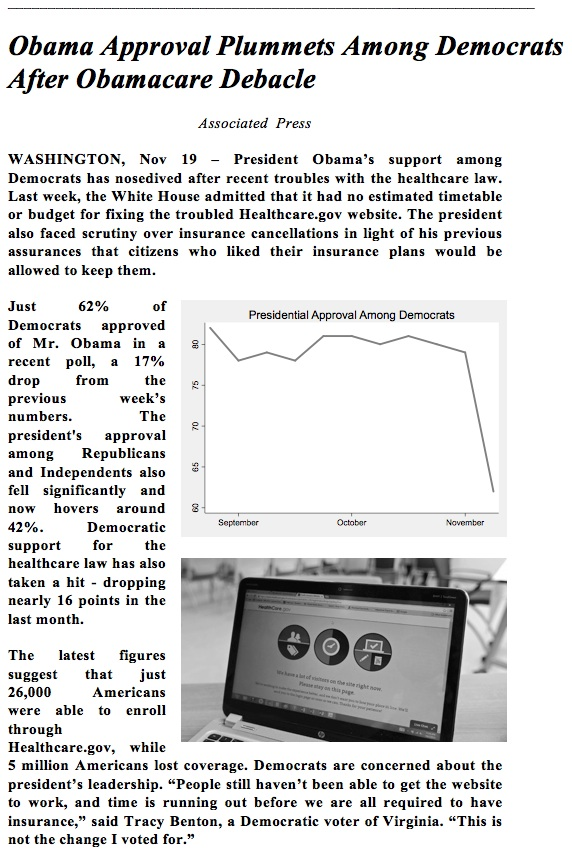
\includegraphics[width=1.05\textwidth]{Dem_C.jpg}
\label{fig:minipage1}
\end{minipage}
\quad
\begin{minipage}[b]{0.45\linewidth}
\caption{Democrats - No Response Condition}
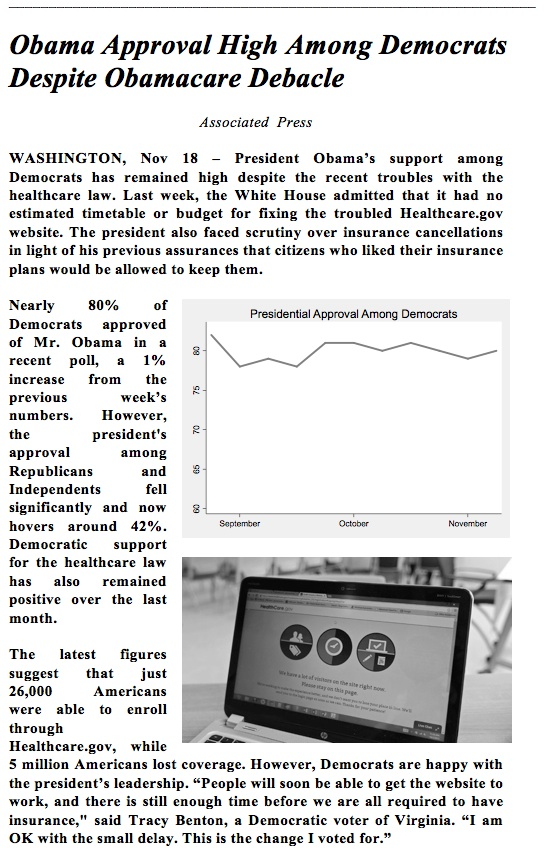
\includegraphics[width=1\textwidth]{Dem_T.jpg}
\label{fig:minipage2}
\end{minipage}
\end{figure}

\begin{figure}[ht]
\centering
\begin{minipage}[b][12cm][b]{0.45\linewidth}
\caption{Republicans - Response Condition}
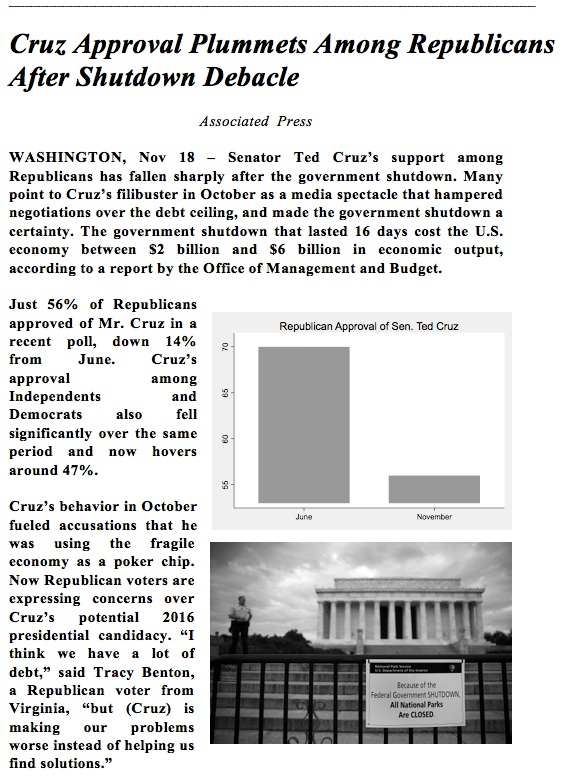
\includegraphics[width=1.05\textwidth]{Rep_C.jpg}
\label{fig:minipage3}
\end{minipage}
\quad
\begin{minipage}[b]{0.45\linewidth}
\caption{Republicans - No Response Condition}
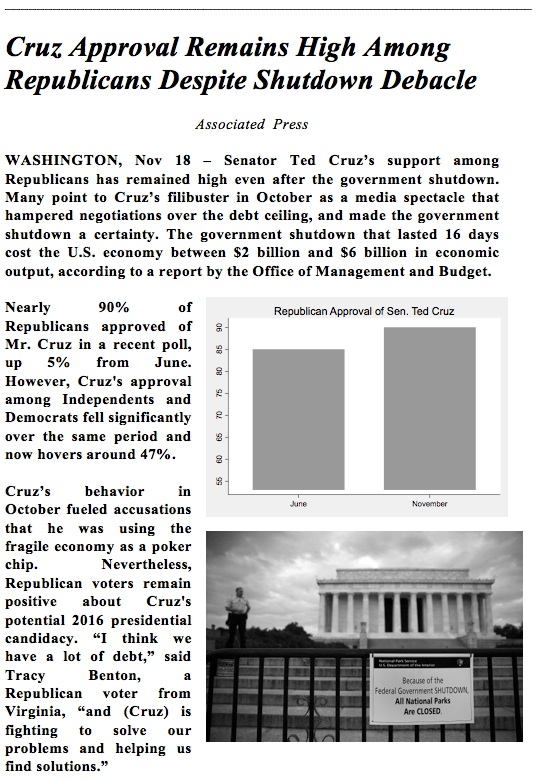
\includegraphics[width=1\textwidth]{Rep_T.jpg}
\label{fig:minipage4}
\end{minipage}
\end{figure}

\begin{figure}[ht]
\centering
\begin{minipage}[b][12cm][b]{0.45\linewidth}
\caption{Control Control}
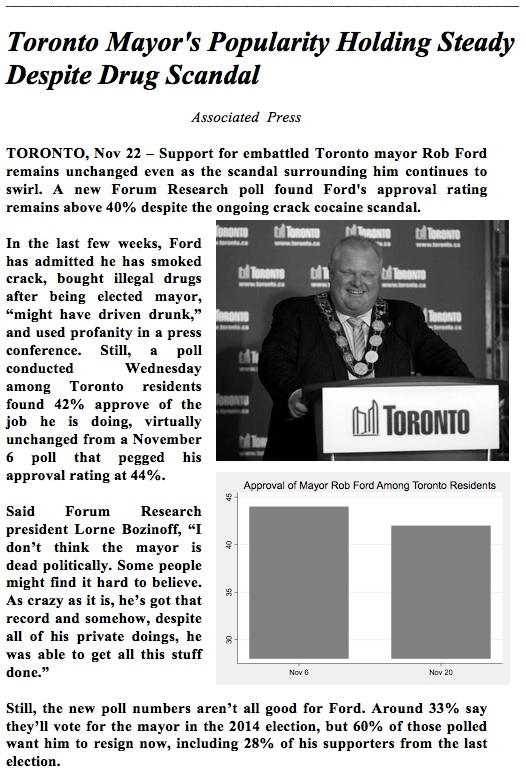
\includegraphics[width=1.05\textwidth]{P.jpg}
\label{fig:minipage5}
\end{minipage}
\end{figure}
\clearpage

\section{Study II Experimental Vignettes}

\begin{figure}[H]
\centering
\captionsetup{font={it}}
\caption{Control Condition}
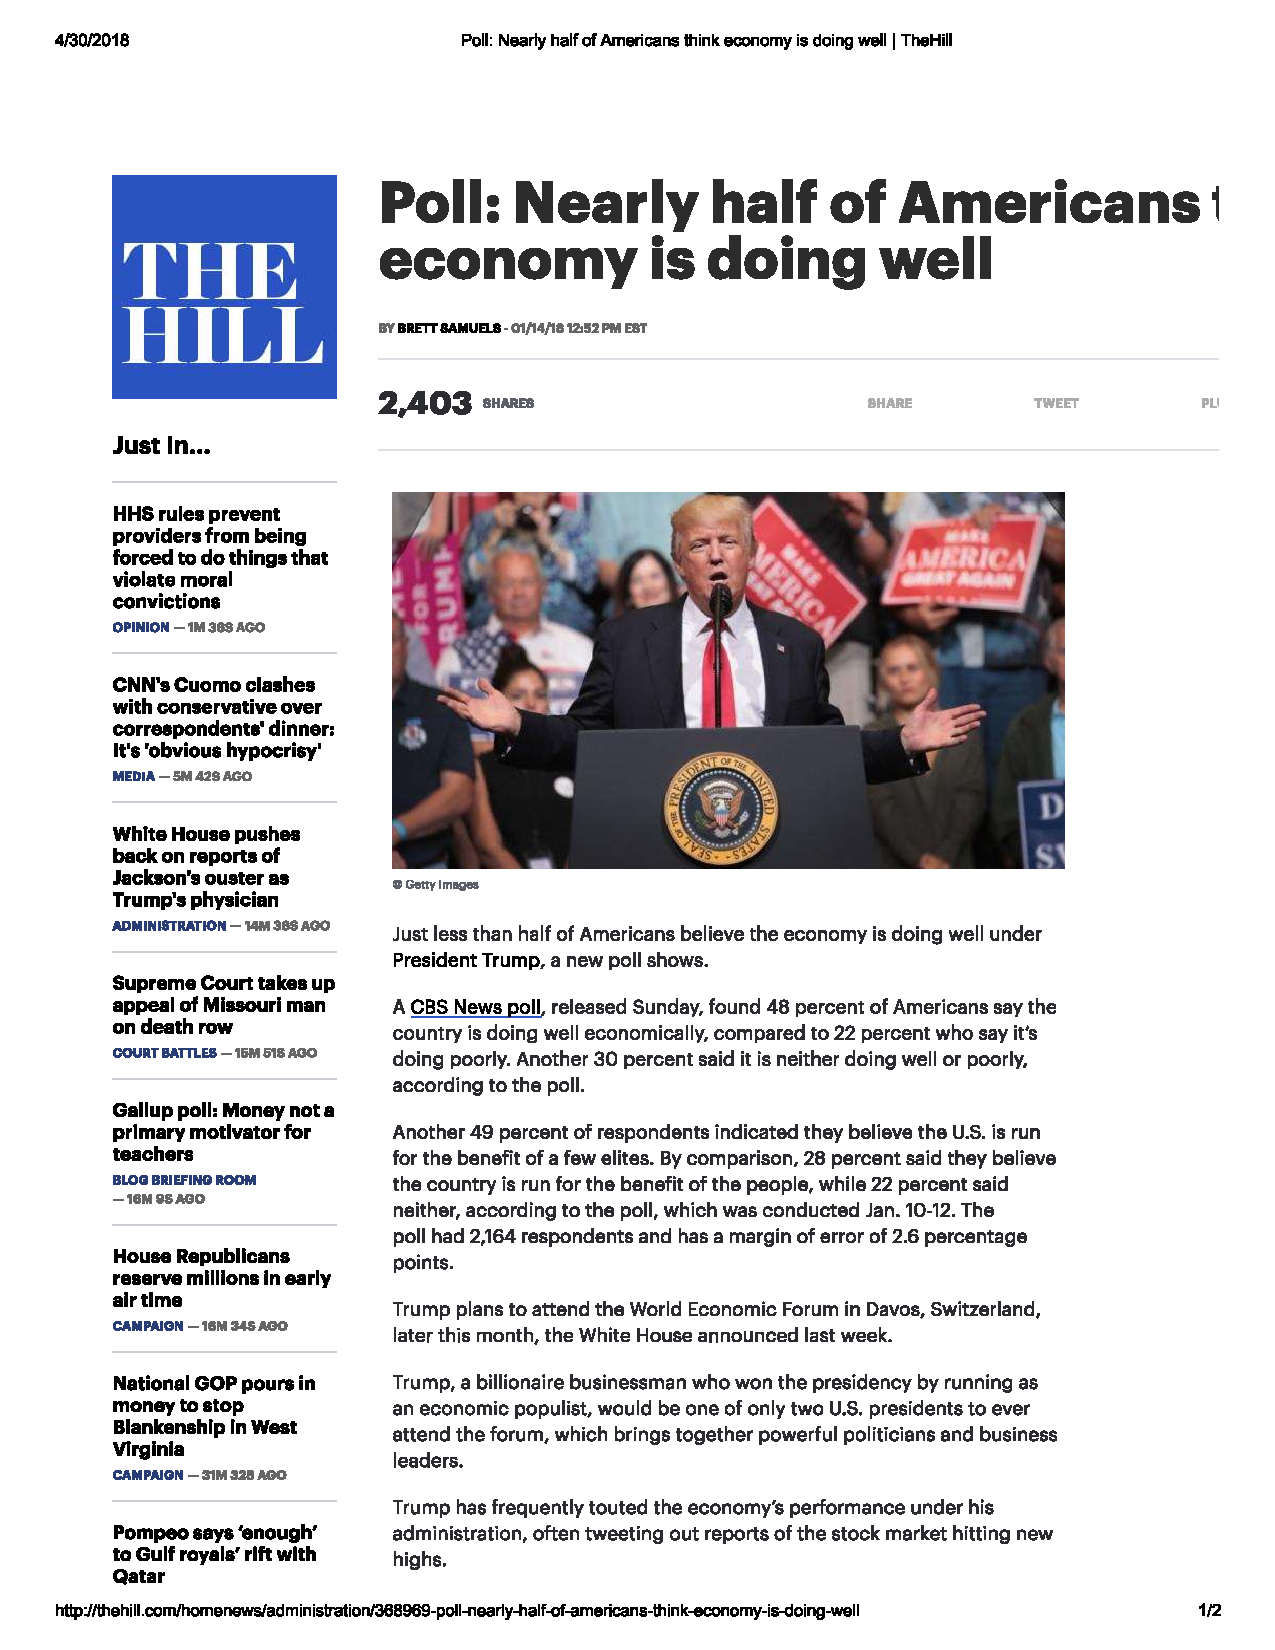
\includegraphics[width=1.05\textwidth]{control.pdf}
\smallskip
\end{figure}

\begin{figure}[H]
\centering
\captionsetup{font={it}}
\caption{Bipartisan Bias Condition}
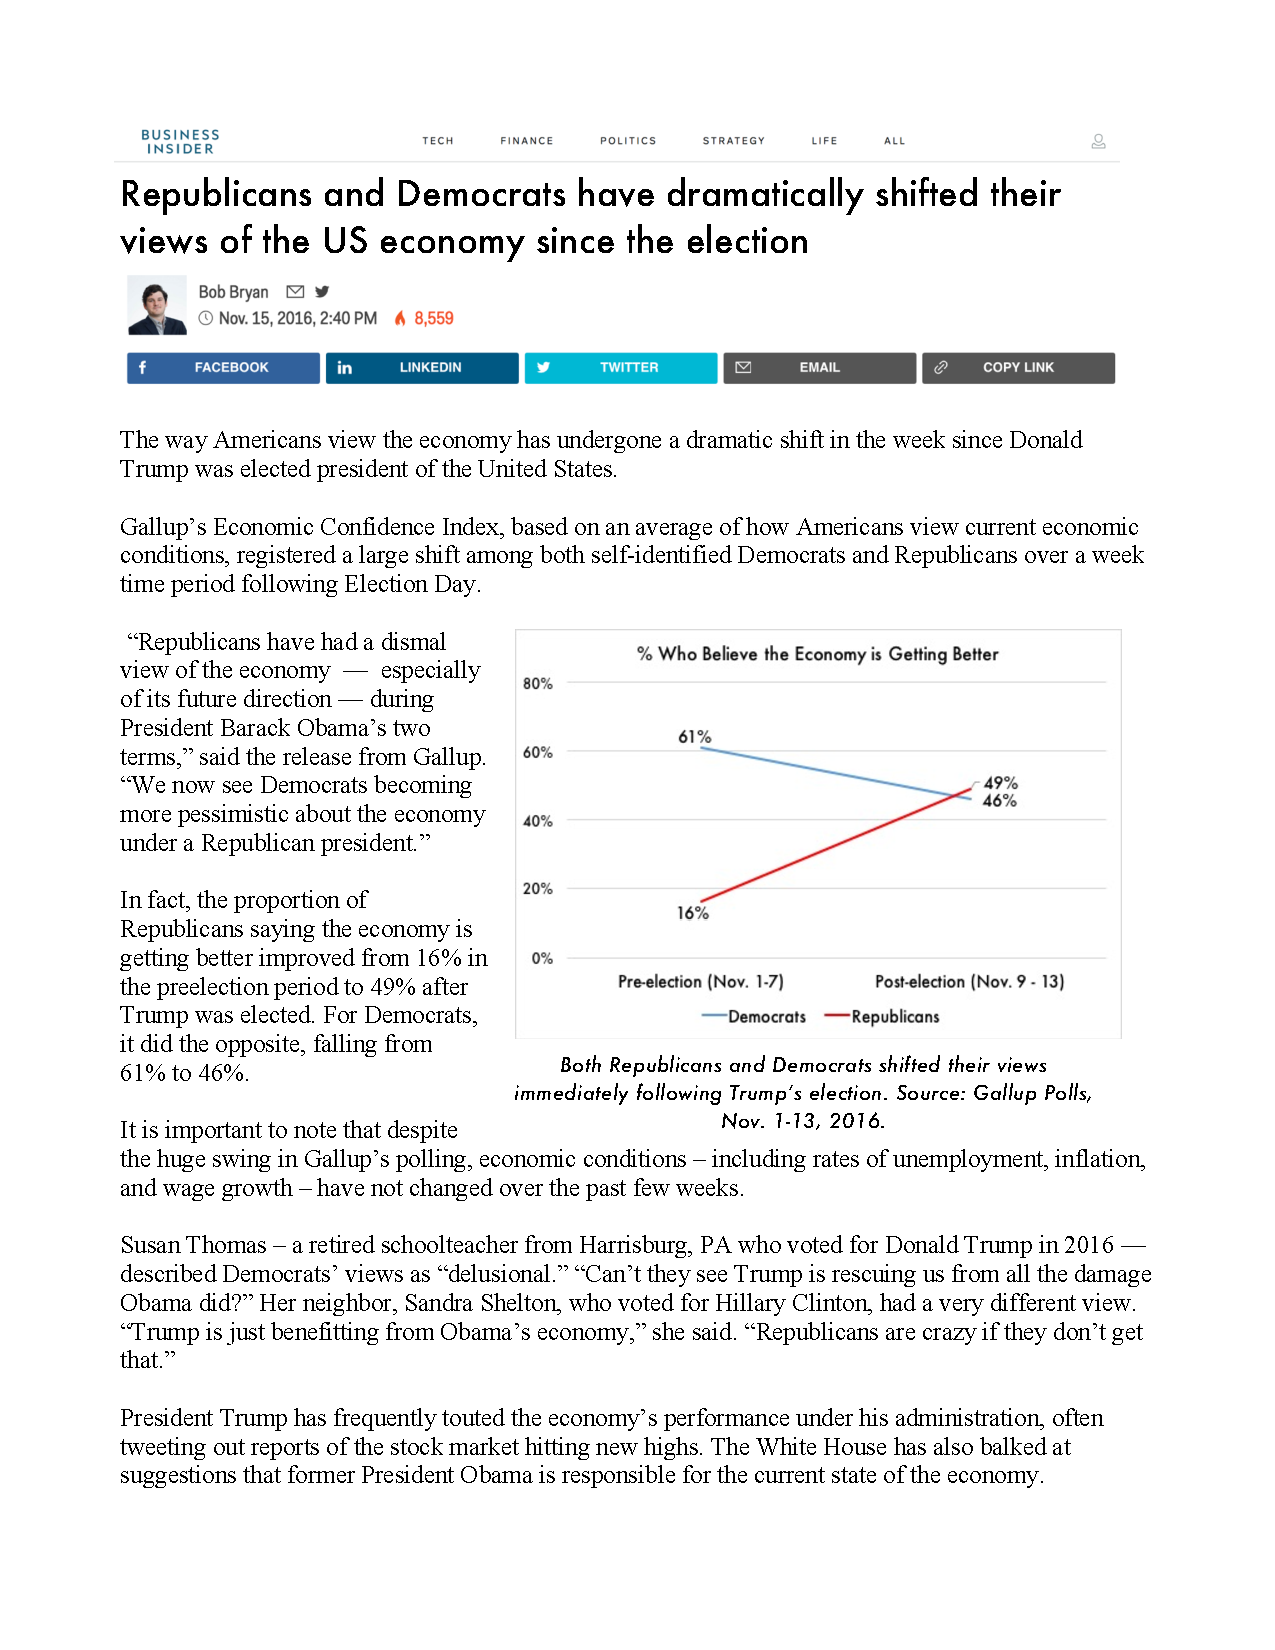
\includegraphics[width=1.05\textwidth]{bipart_motivate.pdf}
\smallskip
\end{figure}


\begin{figure}[H]
\centering
\captionsetup{font={it}}
\caption{Republican Bias Condition}
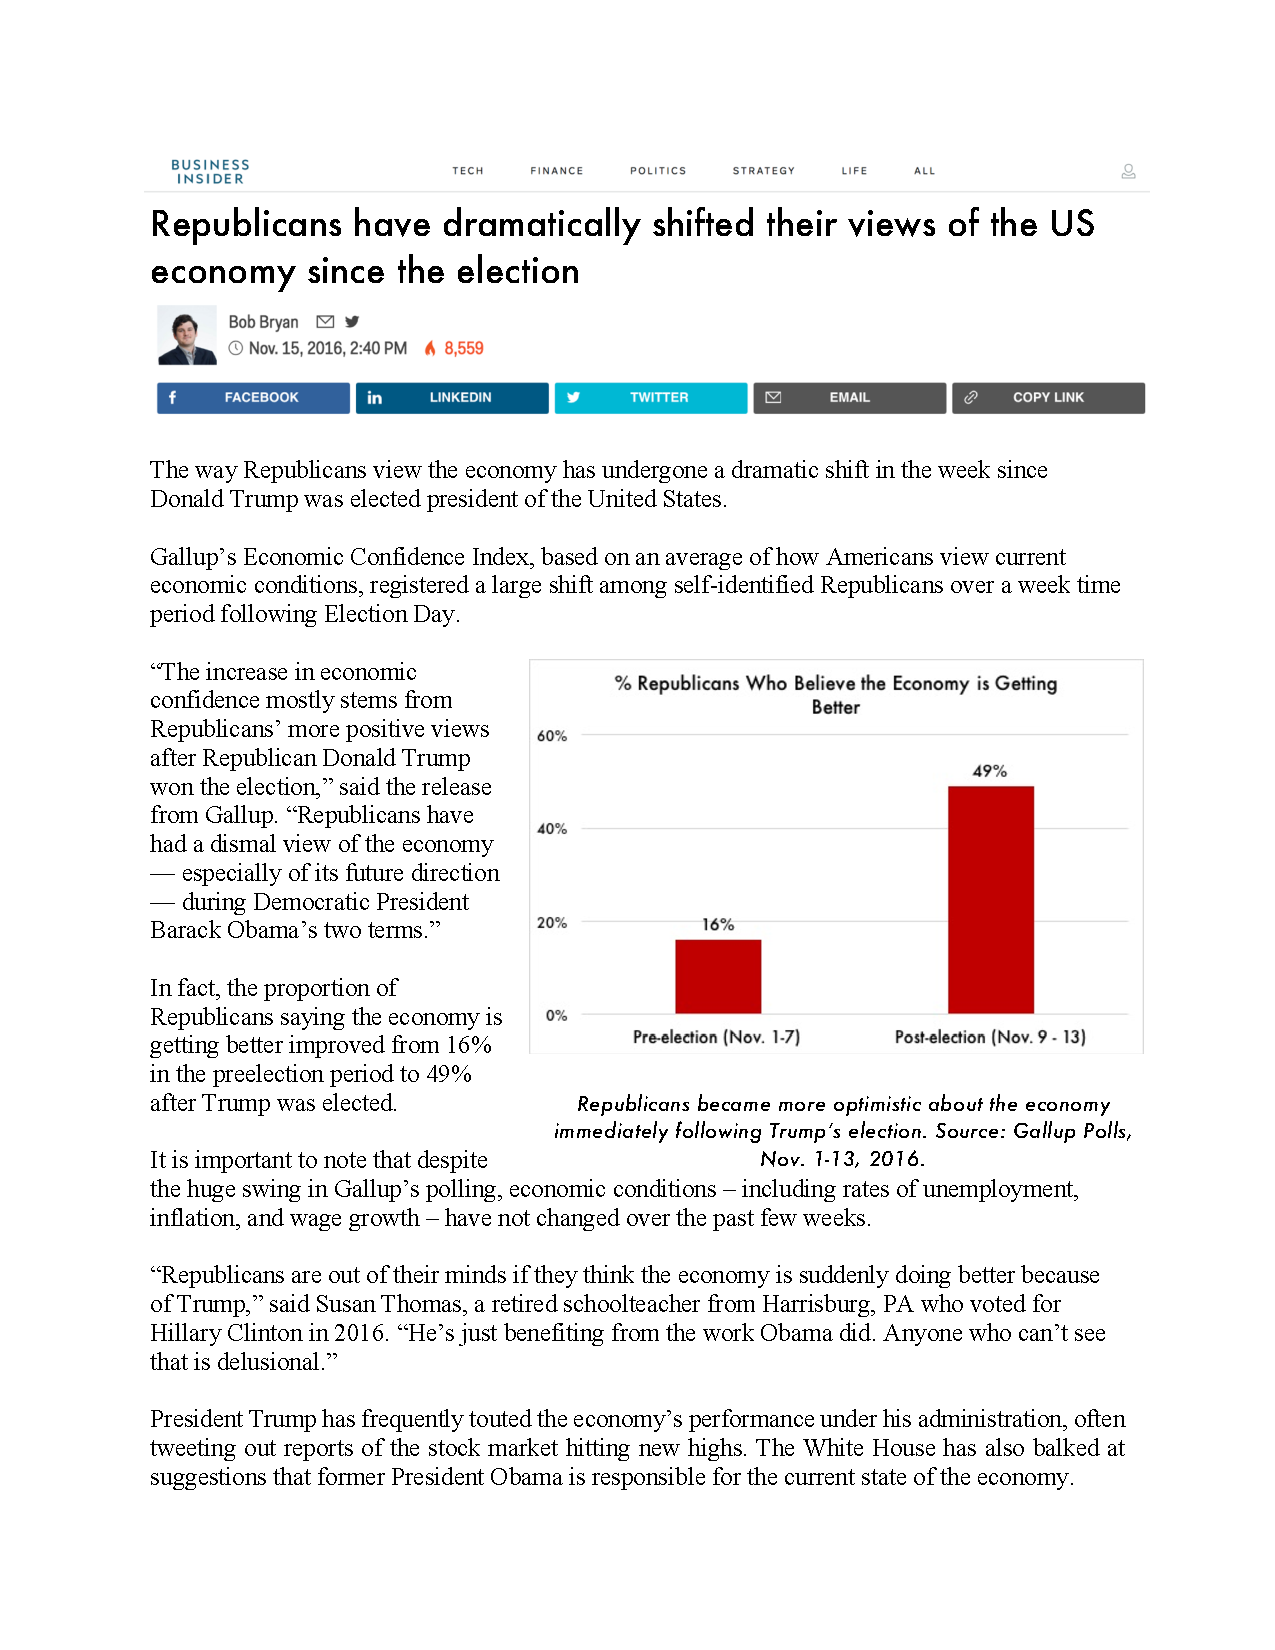
\includegraphics[width=1.05\textwidth]{rep_motivate.pdf}
\smallskip
\end{figure}

\begin{figure}[H]
\centering
\captionsetup{font={it}}
\caption{Democratic Bias Condition}
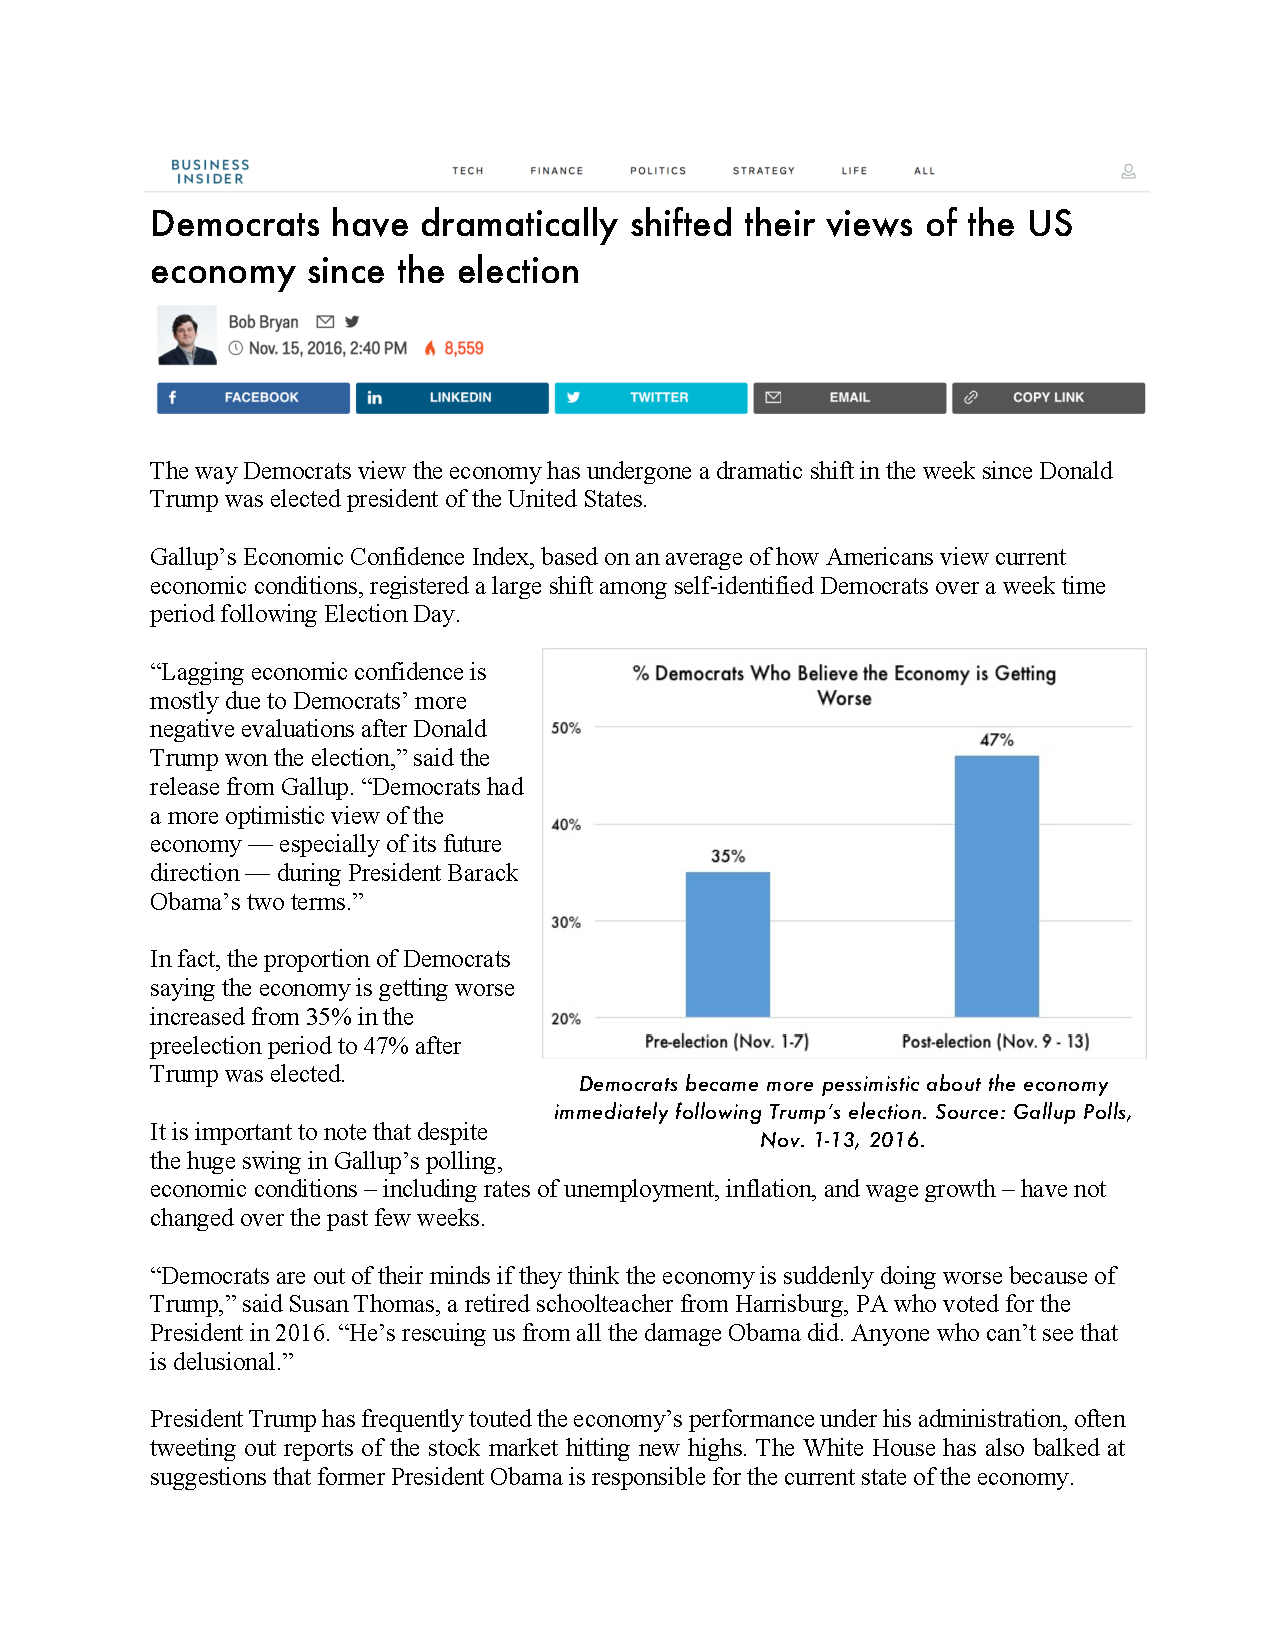
\includegraphics[width=1.05\textwidth]{dem_motivate.pdf}
\smallskip
\end{figure}






\end{document}